\documentclass[1p]{elsarticle_modified}
%\bibliographystyle{elsarticle-num}

%\usepackage[colorlinks]{hyperref}
%\usepackage{abbrmath_seonhwa} %\Abb, \Ascr, \Acal ,\Abf, \Afrak
\usepackage{amsfonts}
\usepackage{amssymb}
\usepackage{amsmath}
\usepackage{amsthm}
\usepackage{scalefnt}
\usepackage{amsbsy}
\usepackage{kotex}
\usepackage{caption}
\usepackage{subfig}
\usepackage{color}
\usepackage{graphicx}
\usepackage{xcolor} %% white, black, red, green, blue, cyan, magenta, yellow
\usepackage{float}
\usepackage{setspace}
\usepackage{hyperref}

\usepackage{tikz}
\usetikzlibrary{arrows}

\usepackage{multirow}
\usepackage{array} % fixed length table
\usepackage{hhline}

%%%%%%%%%%%%%%%%%%%%%
\makeatletter
\renewcommand*\env@matrix[1][\arraystretch]{%
	\edef\arraystretch{#1}%
	\hskip -\arraycolsep
	\let\@ifnextchar\new@ifnextchar
	\array{*\c@MaxMatrixCols c}}
\makeatother %https://tex.stackexchange.com/questions/14071/how-can-i-increase-the-line-spacing-in-a-matrix
%%%%%%%%%%%%%%%

\usepackage[normalem]{ulem}

\newcommand{\msout}[1]{\ifmmode\text{\sout{\ensuremath{#1}}}\else\sout{#1}\fi}
%SOURCE: \msout is \stkout macro in https://tex.stackexchange.com/questions/20609/strikeout-in-math-mode

\newcommand{\cancel}[1]{
	\ifmmode
	{\color{red}\msout{#1}}
	\else
	{\color{red}\sout{#1}}
	\fi
}

\newcommand{\add}[1]{
	{\color{blue}\uwave{#1}}
}

\newcommand{\replace}[2]{
	\ifmmode
	{\color{red}\msout{#1}}{\color{blue}\uwave{#2}}
	\else
	{\color{red}\sout{#1}}{\color{blue}\uwave{#2}}
	\fi
}

\newcommand{\Sol}{\mathcal{S}} %segment
\newcommand{\D}{D} %diagram
\newcommand{\A}{\mathcal{A}} %arc


%%%%%%%%%%%%%%%%%%%%%%%%%%%%%5 test

\def\sl{\operatorname{\textup{SL}}(2,\Cbb)}
\def\psl{\operatorname{\textup{PSL}}(2,\Cbb)}
\def\quan{\mkern 1mu \triangleright \mkern 1mu}

\theoremstyle{definition}
\newtheorem{thm}{Theorem}[section]
\newtheorem{prop}[thm]{Proposition}
\newtheorem{lem}[thm]{Lemma}
\newtheorem{ques}[thm]{Question}
\newtheorem{cor}[thm]{Corollary}
\newtheorem{defn}[thm]{Definition}
\newtheorem{exam}[thm]{Example}
\newtheorem{rmk}[thm]{Remark}
\newtheorem{alg}[thm]{Algorithm}

\newcommand{\I}{\sqrt{-1}}
\begin{document}

%\begin{frontmatter}
%
%\title{Boundary parabolic representations of knots up to 8 crossings}
%
%%% Group authors per affiliation:
%\author{Yunhi Cho} 
%\address{Department of Mathematics, University of Seoul, Seoul, Korea}
%\ead{yhcho@uos.ac.kr}
%
%
%\author{Seonhwa Kim} %\fnref{s_kim}}
%\address{Center for Geometry and Physics, Institute for Basic Science, Pohang, 37673, Korea}
%\ead{ryeona17@ibs.re.kr}
%
%\author{Hyuk Kim}
%\address{Department of Mathematical Sciences, Seoul National University, Seoul 08826, Korea}
%\ead{hyukkim@snu.ac.kr}
%
%\author{Seokbeom Yoon}
%\address{Department of Mathematical Sciences, Seoul National University, Seoul, 08826,  Korea}
%\ead{sbyoon15@snu.ac.kr}
%
%\begin{abstract}
%We find all boundary parabolic representation of knots up to 8 crossings.
%
%\end{abstract}
%\begin{keyword}
%    \MSC[2010] 57M25 
%\end{keyword}
%
%\end{frontmatter}

%\linenumbers
%\tableofcontents
%
\newcommand\colored[1]{\textcolor{white}{\rule[-0.35ex]{0.8em}{1.4ex}}\kern-0.8em\color{red} #1}%
%\newcommand\colored[1]{\textcolor{white}{ #1}\kern-2.17ex	\textcolor{white}{ #1}\kern-1.81ex	\textcolor{white}{ #1}\kern-2.15ex\color{red}#1	}

{\Large $\underline{12n_{0269}~(K12n_{0269})}$}

\setlength{\tabcolsep}{10pt}
\renewcommand{\arraystretch}{1.6}
\vspace{1cm}\begin{tabular}{m{100pt}>{\centering\arraybackslash}m{274pt}}
\multirow{5}{120pt}{
	\centering
	\includegraphics[width=112pt]{../../../GIT/diagram.site/Diagrams/png/2358_12n_0269.png}\\
\ \ \ A knot diagram\footnotemark}&
\allowdisplaybreaks
\textbf{Linearized knot diagam} \\
\cline{2-2}
 &
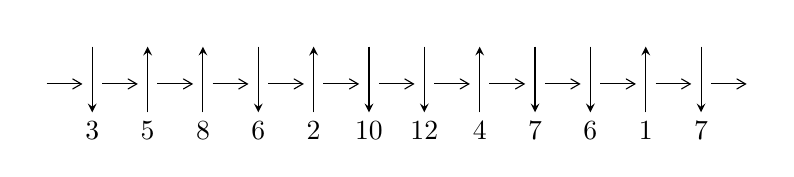
\begin{tikzpicture}[x=20pt, y=17pt]
	% nodes
	\node (C0) at (0, 0) {};
	\node (C1) at (1, 0) {};
	\node (C1U) at (1, +1) {};
	\node (C1D) at (1, -1) {3};

	\node (C2) at (2, 0) {};
	\node (C2U) at (2, +1) {};
	\node (C2D) at (2, -1) {5};

	\node (C3) at (3, 0) {};
	\node (C3U) at (3, +1) {};
	\node (C3D) at (3, -1) {8};

	\node (C4) at (4, 0) {};
	\node (C4U) at (4, +1) {};
	\node (C4D) at (4, -1) {6};

	\node (C5) at (5, 0) {};
	\node (C5U) at (5, +1) {};
	\node (C5D) at (5, -1) {2};

	\node (C6) at (6, 0) {};
	\node (C6U) at (6, +1) {};
	\node (C6D) at (6, -1) {10};

	\node (C7) at (7, 0) {};
	\node (C7U) at (7, +1) {};
	\node (C7D) at (7, -1) {12};

	\node (C8) at (8, 0) {};
	\node (C8U) at (8, +1) {};
	\node (C8D) at (8, -1) {4};

	\node (C9) at (9, 0) {};
	\node (C9U) at (9, +1) {};
	\node (C9D) at (9, -1) {7};

	\node (C10) at (10, 0) {};
	\node (C10U) at (10, +1) {};
	\node (C10D) at (10, -1) {6};

	\node (C11) at (11, 0) {};
	\node (C11U) at (11, +1) {};
	\node (C11D) at (11, -1) {1};

	\node (C12) at (12, 0) {};
	\node (C12U) at (12, +1) {};
	\node (C12D) at (12, -1) {7};
	\node (C13) at (13, 0) {};

	% arrows
	\draw[->,>={angle 60}]
	(C0) edge (C1) (C1) edge (C2) (C2) edge (C3) (C3) edge (C4) (C4) edge (C5) (C5) edge (C6) (C6) edge (C7) (C7) edge (C8) (C8) edge (C9) (C9) edge (C10) (C10) edge (C11) (C11) edge (C12) (C12) edge (C13) ;	\draw[->,>=stealth]
	(C1U) edge (C1D) (C2D) edge (C2U) (C3D) edge (C3U) (C4U) edge (C4D) (C5D) edge (C5U) (C6U) edge (C6D) (C7U) edge (C7D) (C8D) edge (C8U) (C9U) edge (C9D) (C10U) edge (C10D) (C11D) edge (C11U) (C12U) edge (C12D) ;
	\end{tikzpicture} \\
\hhline{~~} \\& 
\textbf{Solving Sequence} \\ \cline{2-2} 
 &
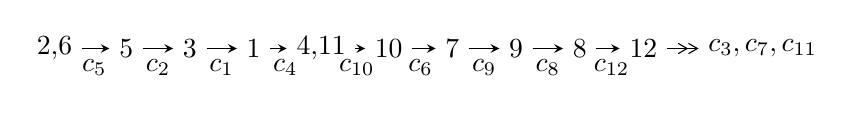
\begin{tikzpicture}[x=23pt, y=7pt]
	% node
	\node (A0) at (-1/8, 0) {2,6};
	\node (A1) at (1, 0) {5};
	\node (A2) at (2, 0) {3};
	\node (A3) at (3, 0) {1};
	\node (A4) at (65/16, 0) {4,11};
	\node (A5) at (41/8, 0) {10};
	\node (A6) at (49/8, 0) {7};
	\node (A7) at (57/8, 0) {9};
	\node (A8) at (65/8, 0) {8};
	\node (A9) at (73/8, 0) {12};
	\node (C1) at (1/2, -1) {$c_{5}$};
	\node (C2) at (3/2, -1) {$c_{2}$};
	\node (C3) at (5/2, -1) {$c_{1}$};
	\node (C4) at (7/2, -1) {$c_{4}$};
	\node (C5) at (37/8, -1) {$c_{10}$};
	\node (C6) at (45/8, -1) {$c_{6}$};
	\node (C7) at (53/8, -1) {$c_{9}$};
	\node (C8) at (61/8, -1) {$c_{8}$};
	\node (C9) at (69/8, -1) {$c_{12}$};
	\node (A10) at (11, 0) {$c_{3},c_{7},c_{11}$};

	% edge
	\draw[->,>=stealth]	
	(A0) edge (A1) (A1) edge (A2) (A2) edge (A3) (A3) edge (A4) (A4) edge (A5) (A5) edge (A6) (A6) edge (A7) (A7) edge (A8) (A8) edge (A9) ;
	\draw[->>,>={angle 60}]	
	(A9) edge (A10);
\end{tikzpicture} \\ 

\end{tabular} \\

\footnotetext{
The image of knot diagram is generated by the software ``\textbf{Draw programme}" developed by Andrew Bartholomew(\url{http://www.layer8.co.uk/maths/draw/index.htm\#Running-draw}), where we modified some parts for our purpose(\url{https://github.com/CATsTAILs/LinksPainter}).
}\phantom \\ \newline 
\centering \textbf{Ideals for irreducible components\footnotemark of $X_{\text{par}}$} 
 
\begin{align*}
I^u_{1}&=\langle 
6075798104 u^{29}-20035573492 u^{28}+\cdots+94573295142 b-102785752178,\\
\phantom{I^u_{1}}&\phantom{= \langle  }52900187657 u^{29}-66435815226 u^{28}+\cdots+189146590284 a-100941534777,\\
\phantom{I^u_{1}}&\phantom{= \langle  }u^{30}-2 u^{29}+\cdots-11 u+4\rangle \\
I^u_{2}&=\langle 
3 u^{18} a-3 u^{18}+\cdots- a-1,\;2 u^{18}-3 u^{17}+\cdots-4 a+5,\;u^{19}- u^{18}+\cdots+2 u+1\rangle \\
I^u_{3}&=\langle 
- u^3+a u- u^2+b+1,\;-2 u^3 a-4 u^2 a+u^3+a^2-4 a u-2 u^2-4 u-5,\;u^4+u^3+u^2+1\rangle \\
I^u_{4}&=\langle 
b-1,\;2 a+2 u+1,\;u^2- u+1\rangle \\
\\
\end{align*}
\raggedright * 4 irreducible components of $\dim_{\mathbb{C}}=0$, with total 78 representations.\\
\footnotetext{All coefficients of polynomials are rational numbers. But the coefficients are sometimes approximated in decimal forms when there is not enough margin.}
\newpage
\renewcommand{\arraystretch}{1}
\centering \section*{I. $I^u_{1}= \langle 6.08\times10^{9} u^{29}-2.00\times10^{10} u^{28}+\cdots+9.46\times10^{10} b-1.03\times10^{11},\;5.29\times10^{10} u^{29}-6.64\times10^{10} u^{28}+\cdots+1.89\times10^{11} a-1.01\times10^{11},\;u^{30}-2 u^{29}+\cdots-11 u+4 \rangle$}
\flushleft \textbf{(i) Arc colorings}\\
\begin{tabular}{m{7pt} m{180pt} m{7pt} m{180pt} }
\flushright $a_{2}=$&$\begin{pmatrix}0\\u\end{pmatrix}$ \\
\flushright $a_{6}=$&$\begin{pmatrix}1\\0\end{pmatrix}$ \\
\flushright $a_{5}=$&$\begin{pmatrix}1\\u^2\end{pmatrix}$ \\
\flushright $a_{3}=$&$\begin{pmatrix}u\\u^3+u\end{pmatrix}$ \\
\flushright $a_{1}=$&$\begin{pmatrix}u^3\\u^5+u^3+u\end{pmatrix}$ \\
\flushright $a_{4}=$&$\begin{pmatrix}u^2+1\\u^2\end{pmatrix}$ \\
\flushright $a_{11}=$&$\begin{pmatrix}-0.279678 u^{29}+0.351240 u^{28}+\cdots-2.48757 u+0.533668\\-0.0642443 u^{29}+0.211852 u^{28}+\cdots-0.962626 u+1.08684\end{pmatrix}$ \\
\flushright $a_{10}=$&$\begin{pmatrix}-0.343923 u^{29}+0.563092 u^{28}+\cdots-3.45020 u+1.62051\\-0.0642443 u^{29}+0.211852 u^{28}+\cdots-0.962626 u+1.08684\end{pmatrix}$ \\
\flushright $a_{7}=$&$\begin{pmatrix}-0.293504 u^{29}+0.578779 u^{28}+\cdots-3.77569 u+2.01661\\-0.0196924 u^{29}+0.238501 u^{28}+\cdots-1.68736 u+1.14206\end{pmatrix}$ \\
\flushright $a_{9}=$&$\begin{pmatrix}-0.642162 u^{29}+1.14610 u^{28}+\cdots-7.29055 u+2.93572\\-0.0853310 u^{29}+0.458919 u^{28}+\cdots-2.98810 u+2.09785\end{pmatrix}$ \\
\flushright $a_{8}=$&$\begin{pmatrix}-0.565573 u^{29}+1.10421 u^{28}+\cdots-7.29137 u+2.70821\\-0.0269374 u^{29}+0.494525 u^{28}+\cdots-3.51309 u+2.26229\end{pmatrix}$ \\
\flushright $a_{12}=$&$\begin{pmatrix}-0.298240 u^{29}+0.583012 u^{28}+\cdots-3.84035 u+1.31521\\-0.0210866 u^{29}+0.247066 u^{28}+\cdots-1.02547 u+1.01102\end{pmatrix}$\\&\end{tabular}
\flushleft \textbf{(ii) Obstruction class $= -1$}\\~\\
\flushleft \textbf{(iii) Cusp Shapes $= \frac{13126781461}{15762215857} u^{29}-\frac{346887419065}{189146590284} u^{28}+\cdots+\frac{2455780116659}{189146590284} u-\frac{364257663059}{47286647571}$}\\~\\
\newpage\renewcommand{\arraystretch}{1}
\flushleft \textbf{(iv) u-Polynomials at the component}\newline \\
\begin{tabular}{m{50pt}|m{274pt}}
Crossings & \hspace{64pt}u-Polynomials at each crossing \\
\hline $$\begin{aligned}c_{1},c_{4}\end{aligned}$$&$\begin{aligned}
&u^{30}+10 u^{29}+\cdots- u+16
\end{aligned}$\\
\hline $$\begin{aligned}c_{2},c_{5}\end{aligned}$$&$\begin{aligned}
&u^{30}+2 u^{29}+\cdots+11 u+4
\end{aligned}$\\
\hline $$\begin{aligned}c_{3},c_{8}\end{aligned}$$&$\begin{aligned}
&u^{30}-3 u^{29}+\cdots+24 u+32
\end{aligned}$\\
\hline $$\begin{aligned}c_{6},c_{7},c_{9}\\c_{10},c_{12}\end{aligned}$$&$\begin{aligned}
&u^{30}+2 u^{29}+\cdots- u+1
\end{aligned}$\\
\hline $$\begin{aligned}c_{11}\end{aligned}$$&$\begin{aligned}
&u^{30}-8 u^{29}+\cdots-15 u+1
\end{aligned}$\\
\hline
\end{tabular}\\~\\
\newpage\renewcommand{\arraystretch}{1}
\flushleft \textbf{(v) Riley Polynomials at the component}\newline \\
\begin{tabular}{m{50pt}|m{274pt}}
Crossings & \hspace{64pt}Riley Polynomials at each crossing \\
\hline $$\begin{aligned}c_{1},c_{4}\end{aligned}$$&$\begin{aligned}
&y^{30}+22 y^{29}+\cdots+3743 y+256
\end{aligned}$\\
\hline $$\begin{aligned}c_{2},c_{5}\end{aligned}$$&$\begin{aligned}
&y^{30}+10 y^{29}+\cdots- y+16
\end{aligned}$\\
\hline $$\begin{aligned}c_{3},c_{8}\end{aligned}$$&$\begin{aligned}
&y^{30}-15 y^{29}+\cdots-6336 y+1024
\end{aligned}$\\
\hline $$\begin{aligned}c_{6},c_{7},c_{9}\\c_{10},c_{12}\end{aligned}$$&$\begin{aligned}
&y^{30}+8 y^{29}+\cdots+15 y+1
\end{aligned}$\\
\hline $$\begin{aligned}c_{11}\end{aligned}$$&$\begin{aligned}
&y^{30}+24 y^{29}+\cdots+19 y+1
\end{aligned}$\\
\hline
\end{tabular}\\~\\
\newpage\flushleft \textbf{(vi) Complex Volumes and Cusp Shapes}
$$\begin{array}{c|c|c}  
\text{Solutions to }I^u_{1}& \I (\text{vol} + \sqrt{-1}CS) & \text{Cusp shape}\\
 \hline 
\begin{aligned}
u &= -0.460643 + 0.958497 I \\
a &= \phantom{-}1.032200 - 0.246838 I \\
b &= -0.299080 - 0.268098 I\end{aligned}
 & -0.32179 - 2.57657 I & \phantom{-}1.59153 + 5.16266 I \\ \hline\begin{aligned}
u &= -0.460643 - 0.958497 I \\
a &= \phantom{-}1.032200 + 0.246838 I \\
b &= -0.299080 + 0.268098 I\end{aligned}
 & -0.32179 + 2.57657 I & \phantom{-}1.59153 - 5.16266 I \\ \hline\begin{aligned}
u &= \phantom{-}0.117766 + 1.065450 I \\
a &= -2.08067 + 0.32615 I \\
b &= \phantom{-}0.868345 - 0.853291 I\end{aligned}
 & -5.22441 + 3.04204 I & -6.16892 - 2.76702 I \\ \hline\begin{aligned}
u &= \phantom{-}0.117766 - 1.065450 I \\
a &= -2.08067 - 0.32615 I \\
b &= \phantom{-}0.868345 + 0.853291 I\end{aligned}
 & -5.22441 - 3.04204 I & -6.16892 + 2.76702 I \\ \hline\begin{aligned}
u &= \phantom{-}0.892544 + 0.608188 I \\
a &= \phantom{-}0.357885 - 0.459993 I \\
b &= -0.660894 - 1.208280 I\end{aligned}
 & \phantom{-}3.48880 - 10.37700 I & \phantom{-}3.38979 + 5.72342 I \\ \hline\begin{aligned}
u &= \phantom{-}0.892544 - 0.608188 I \\
a &= \phantom{-}0.357885 + 0.459993 I \\
b &= -0.660894 + 1.208280 I\end{aligned}
 & \phantom{-}3.48880 + 10.37700 I & \phantom{-}3.38979 - 5.72342 I \\ \hline\begin{aligned}
u &= -0.835530 + 0.693005 I \\
a &= -0.118947 - 0.761630 I \\
b &= \phantom{-}0.596590 - 0.966034 I\end{aligned}
 & \phantom{-}1.29700 + 3.10575 I & \phantom{-}1.45147 - 3.18731 I \\ \hline\begin{aligned}
u &= -0.835530 - 0.693005 I \\
a &= -0.118947 + 0.761630 I \\
b &= \phantom{-}0.596590 + 0.966034 I\end{aligned}
 & \phantom{-}1.29700 - 3.10575 I & \phantom{-}1.45147 + 3.18731 I \\ \hline\begin{aligned}
u &= \phantom{-}0.513340 + 0.739634 I \\
a &= -1.14053 - 0.97145 I \\
b &= \phantom{-}1.145550 - 0.289264 I\end{aligned}
 & -1.57253 + 1.48061 I & \phantom{-}1.51311 + 5.82808 I \\ \hline\begin{aligned}
u &= \phantom{-}0.513340 - 0.739634 I \\
a &= -1.14053 + 0.97145 I \\
b &= \phantom{-}1.145550 + 0.289264 I\end{aligned}
 & -1.57253 - 1.48061 I & \phantom{-}1.51311 - 5.82808 I\\
 \hline 
 \end{array}$$\newpage$$\begin{array}{c|c|c}  
\text{Solutions to }I^u_{1}& \I (\text{vol} + \sqrt{-1}CS) & \text{Cusp shape}\\
 \hline 
\begin{aligned}
u &= -0.850935 + 0.293187 I \\
a &= \phantom{-}0.444169 - 0.489109 I \\
b &= -0.601963 - 1.009720 I\end{aligned}
 & \phantom{-}1.66857 - 6.29086 I & \phantom{-}3.10303 + 6.83080 I \\ \hline\begin{aligned}
u &= -0.850935 - 0.293187 I \\
a &= \phantom{-}0.444169 + 0.489109 I \\
b &= -0.601963 + 1.009720 I\end{aligned}
 & \phantom{-}1.66857 + 6.29086 I & \phantom{-}3.10303 - 6.83080 I \\ \hline\begin{aligned}
u &= \phantom{-}0.590492 + 0.982207 I \\
a &= -0.644113 - 1.170090 I \\
b &= \phantom{-}1.149850 + 0.591978 I\end{aligned}
 & -2.48088 + 3.02207 I & -2.21456 - 6.76782 I \\ \hline\begin{aligned}
u &= \phantom{-}0.590492 - 0.982207 I \\
a &= -0.644113 + 1.170090 I \\
b &= \phantom{-}1.149850 - 0.591978 I\end{aligned}
 & -2.48088 - 3.02207 I & -2.21456 + 6.76782 I \\ \hline\begin{aligned}
u &= -0.120227 + 1.185320 I \\
a &= \phantom{-}1.71764 + 0.85667 I \\
b &= -0.727551 - 1.085270 I\end{aligned}
 & -3.53890 - 9.16679 I & -2.72882 + 7.28806 I \\ \hline\begin{aligned}
u &= -0.120227 - 1.185320 I \\
a &= \phantom{-}1.71764 - 0.85667 I \\
b &= -0.727551 + 1.085270 I\end{aligned}
 & -3.53890 + 9.16679 I & -2.72882 - 7.28806 I \\ \hline\begin{aligned}
u &= -0.537667 + 0.602506 I \\
a &= \phantom{-}0.295236 + 0.519101 I \\
b &= \phantom{-}0.023047 + 0.423163 I\end{aligned}
 & \phantom{-}0.81059 - 1.39109 I & \phantom{-}1.55512 + 4.14990 I \\ \hline\begin{aligned}
u &= -0.537667 - 0.602506 I \\
a &= \phantom{-}0.295236 - 0.519101 I \\
b &= \phantom{-}0.023047 - 0.423163 I\end{aligned}
 & \phantom{-}0.81059 + 1.39109 I & \phantom{-}1.55512 - 4.14990 I \\ \hline\begin{aligned}
u &= -0.530973 + 1.119350 I \\
a &= \phantom{-}0.144119 - 0.924498 I \\
b &= -0.645054 + 0.883761 I\end{aligned}
 & -0.91910 + 1.29166 I & -0.69831 - 3.06877 I \\ \hline\begin{aligned}
u &= -0.530973 - 1.119350 I \\
a &= \phantom{-}0.144119 + 0.924498 I \\
b &= -0.645054 - 0.883761 I\end{aligned}
 & -0.91910 - 1.29166 I & -0.69831 + 3.06877 I\\
 \hline 
 \end{array}$$\newpage$$\begin{array}{c|c|c}  
\text{Solutions to }I^u_{1}& \I (\text{vol} + \sqrt{-1}CS) & \text{Cusp shape}\\
 \hline 
\begin{aligned}
u &= -0.730890 + 1.026770 I \\
a &= -1.64352 + 1.06510 I \\
b &= \phantom{-}0.646060 + 1.041760 I\end{aligned}
 & \phantom{-}0.26873 - 8.97735 I & \phantom{-}0.28174 + 7.42318 I \\ \hline\begin{aligned}
u &= -0.730890 - 1.026770 I \\
a &= -1.64352 - 1.06510 I \\
b &= \phantom{-}0.646060 - 1.041760 I\end{aligned}
 & \phantom{-}0.26873 + 8.97735 I & \phantom{-}0.28174 - 7.42318 I \\ \hline\begin{aligned}
u &= \phantom{-}0.896688 + 0.897515 I \\
a &= \phantom{-}0.544249 + 0.743729 I \\
b &= -0.269532 + 0.876061 I\end{aligned}
 & \phantom{-}9.52166 + 4.35690 I & \phantom{-}1.93733 - 9.19475 I \\ \hline\begin{aligned}
u &= \phantom{-}0.896688 - 0.897515 I \\
a &= \phantom{-}0.544249 - 0.743729 I \\
b &= -0.269532 - 0.876061 I\end{aligned}
 & \phantom{-}9.52166 - 4.35690 I & \phantom{-}1.93733 + 9.19475 I \\ \hline\begin{aligned}
u &= \phantom{-}0.875554 + 0.943207 I \\
a &= -0.406635 - 0.439577 I \\
b &= -0.231064 - 0.841743 I\end{aligned}
 & \phantom{-}9.37686 + 2.17701 I & \phantom{-}0.69666 + 4.17919 I \\ \hline\begin{aligned}
u &= \phantom{-}0.875554 - 0.943207 I \\
a &= -0.406635 + 0.439577 I \\
b &= -0.231064 + 0.841743 I\end{aligned}
 & \phantom{-}9.37686 - 2.17701 I & \phantom{-}0.69666 - 4.17919 I \\ \hline\begin{aligned}
u &= \phantom{-}0.719689 + 1.077380 I \\
a &= \phantom{-}2.03341 + 0.65165 I \\
b &= -0.70309 + 1.23931 I\end{aligned}
 & \phantom{-}2.0453 + 16.3438 I & \phantom{-}1.41001 - 9.88978 I \\ \hline\begin{aligned}
u &= \phantom{-}0.719689 - 1.077380 I \\
a &= \phantom{-}2.03341 - 0.65165 I \\
b &= -0.70309 - 1.23931 I\end{aligned}
 & \phantom{-}2.0453 - 16.3438 I & \phantom{-}1.41001 + 9.88978 I \\ \hline\begin{aligned}
u &= \phantom{-}0.460792 + 0.211623 I \\
a &= -0.159496 - 1.172690 I \\
b &= \phantom{-}0.708800 - 0.487048 I\end{aligned}
 & -1.26041 + 1.13919 I & -3.24420 - 2.21188 I \\ \hline\begin{aligned}
u &= \phantom{-}0.460792 - 0.211623 I \\
a &= -0.159496 + 1.172690 I \\
b &= \phantom{-}0.708800 + 0.487048 I\end{aligned}
 & -1.26041 - 1.13919 I & -3.24420 + 2.21188 I\\
 \hline 
 \end{array}$$\newpage\newpage\renewcommand{\arraystretch}{1}
\centering \section*{II. $I^u_{2}= \langle 3 u^{18} a-3 u^{18}+\cdots- a-1,\;2 u^{18}-3 u^{17}+\cdots-4 a+5,\;u^{19}- u^{18}+\cdots+2 u+1 \rangle$}
\flushleft \textbf{(i) Arc colorings}\\
\begin{tabular}{m{7pt} m{180pt} m{7pt} m{180pt} }
\flushright $a_{2}=$&$\begin{pmatrix}0\\u\end{pmatrix}$ \\
\flushright $a_{6}=$&$\begin{pmatrix}1\\0\end{pmatrix}$ \\
\flushright $a_{5}=$&$\begin{pmatrix}1\\u^2\end{pmatrix}$ \\
\flushright $a_{3}=$&$\begin{pmatrix}u\\u^3+u\end{pmatrix}$ \\
\flushright $a_{1}=$&$\begin{pmatrix}u^3\\u^5+u^3+u\end{pmatrix}$ \\
\flushright $a_{4}=$&$\begin{pmatrix}u^2+1\\u^2\end{pmatrix}$ \\
\flushright $a_{11}=$&$\begin{pmatrix}a\\-\frac{3}{2} u^{18} a+\frac{3}{2} u^{18}+\cdots+\frac{1}{2} a+\frac{1}{2}\end{pmatrix}$ \\
\flushright $a_{10}=$&$\begin{pmatrix}-\frac{3}{2} u^{18} a+\frac{3}{2} u^{18}+\cdots+\frac{3}{2} a+\frac{1}{2}\\-\frac{3}{2} u^{18} a+\frac{3}{2} u^{18}+\cdots+\frac{1}{2} a+\frac{1}{2}\end{pmatrix}$ \\
\flushright $a_{7}=$&$\begin{pmatrix}2 u^{17} a- u^{17}+\cdots- a+4\\\frac{3}{2} u^{18} a-\frac{3}{2} u^{18}+\cdots-\frac{1}{2} a-\frac{1}{2}\end{pmatrix}$ \\
\flushright $a_{9}=$&$\begin{pmatrix}- u^{13}-2 u^{11}-3 u^9-2 u^7+u\\- u^{15}-3 u^{13}-6 u^{11}-7 u^9-6 u^7-4 u^5-2 u^3- u\end{pmatrix}$ \\
\flushright $a_{8}=$&$\begin{pmatrix}u^{18}+3 u^{16}+6 u^{14}+7 u^{12}+5 u^{10}+3 u^8- u^2-1\\u^{18}- u^{17}+\cdots-3 u-1\end{pmatrix}$ \\
\flushright $a_{12}=$&$\begin{pmatrix}-\frac{1}{2} u^{18} a+\frac{3}{2} u^{18}+\cdots+\frac{1}{2} a-\frac{1}{2}\\-2 u^{18} a+3 u^{18}+\cdots+a u-4 u\end{pmatrix}$\\&\end{tabular}
\flushleft \textbf{(ii) Obstruction class $= -1$}\\~\\
\flushleft \textbf{(iii) Cusp Shapes $= -4 u^{17}+4 u^{16}-12 u^{15}+12 u^{14}-28 u^{13}+24 u^{12}-36 u^{11}+32 u^{10}-36 u^9+28 u^8-28 u^7+28 u^6-12 u^5+16 u^4-12 u^3+12 u^2+4 u+6$}\\~\\
\newpage\renewcommand{\arraystretch}{1}
\flushleft \textbf{(iv) u-Polynomials at the component}\newline \\
\begin{tabular}{m{50pt}|m{274pt}}
Crossings & \hspace{64pt}u-Polynomials at each crossing \\
\hline $$\begin{aligned}c_{1},c_{4}\end{aligned}$$&$\begin{aligned}
&(u^{19}+7 u^{18}+\cdots+2 u-1)^{2}
\end{aligned}$\\
\hline $$\begin{aligned}c_{2},c_{5}\end{aligned}$$&$\begin{aligned}
&(u^{19}+u^{18}+\cdots+2 u-1)^{2}
\end{aligned}$\\
\hline $$\begin{aligned}c_{3},c_{8}\end{aligned}$$&$\begin{aligned}
&(u^{19}+u^{18}+\cdots- u^2+1)^{2}
\end{aligned}$\\
\hline $$\begin{aligned}c_{6},c_{7},c_{9}\\c_{10},c_{12}\end{aligned}$$&$\begin{aligned}
&u^{38}-5 u^{37}+\cdots-173 u+34
\end{aligned}$\\
\hline $$\begin{aligned}c_{11}\end{aligned}$$&$\begin{aligned}
&u^{38}-19 u^{37}+\cdots-13387 u+1156
\end{aligned}$\\
\hline
\end{tabular}\\~\\
\newpage\renewcommand{\arraystretch}{1}
\flushleft \textbf{(v) Riley Polynomials at the component}\newline \\
\begin{tabular}{m{50pt}|m{274pt}}
Crossings & \hspace{64pt}Riley Polynomials at each crossing \\
\hline $$\begin{aligned}c_{1},c_{4}\end{aligned}$$&$\begin{aligned}
&(y^{19}+11 y^{18}+\cdots+42 y-1)^{2}
\end{aligned}$\\
\hline $$\begin{aligned}c_{2},c_{5}\end{aligned}$$&$\begin{aligned}
&(y^{19}+7 y^{18}+\cdots+2 y-1)^{2}
\end{aligned}$\\
\hline $$\begin{aligned}c_{3},c_{8}\end{aligned}$$&$\begin{aligned}
&(y^{19}-5 y^{18}+\cdots+2 y-1)^{2}
\end{aligned}$\\
\hline $$\begin{aligned}c_{6},c_{7},c_{9}\\c_{10},c_{12}\end{aligned}$$&$\begin{aligned}
&y^{38}+19 y^{37}+\cdots+13387 y+1156
\end{aligned}$\\
\hline $$\begin{aligned}c_{11}\end{aligned}$$&$\begin{aligned}
&y^{38}- y^{37}+\cdots+7530783 y+1336336
\end{aligned}$\\
\hline
\end{tabular}\\~\\
\newpage\flushleft \textbf{(vi) Complex Volumes and Cusp Shapes}
$$\begin{array}{c|c|c}  
\text{Solutions to }I^u_{2}& \I (\text{vol} + \sqrt{-1}CS) & \text{Cusp shape}\\
 \hline 
\begin{aligned}
u &= \phantom{-}0.787239 + 0.559366 I \\
a &= \phantom{-}0.516479 + 0.470519 I \\
b &= -0.991761 + 0.337645 I\end{aligned}
 & \phantom{-}0.85217 - 4.39903 I & \phantom{-}0.93348 + 2.80289 I \\ \hline\begin{aligned}
u &= \phantom{-}0.787239 + 0.559366 I \\
a &= -0.195675 + 0.232139 I \\
b &= \phantom{-}0.689098 + 1.130990 I\end{aligned}
 & \phantom{-}0.85217 - 4.39903 I & \phantom{-}0.93348 + 2.80289 I \\ \hline\begin{aligned}
u &= \phantom{-}0.787239 - 0.559366 I \\
a &= \phantom{-}0.516479 - 0.470519 I \\
b &= -0.991761 - 0.337645 I\end{aligned}
 & \phantom{-}0.85217 + 4.39903 I & \phantom{-}0.93348 - 2.80289 I \\ \hline\begin{aligned}
u &= \phantom{-}0.787239 - 0.559366 I \\
a &= -0.195675 - 0.232139 I \\
b &= \phantom{-}0.689098 - 1.130990 I\end{aligned}
 & \phantom{-}0.85217 + 4.39903 I & \phantom{-}0.93348 - 2.80289 I \\ \hline\begin{aligned}
u &= \phantom{-}0.709462 + 0.766103 I \\
a &= \phantom{-}0.585393 + 0.482577 I \\
b &= -0.678167 - 0.996758 I\end{aligned}
 & \phantom{-}6.91199 - 0.16816 I & \phantom{-}6.16829 + 0.91431 I \\ \hline\begin{aligned}
u &= \phantom{-}0.709462 + 0.766103 I \\
a &= \phantom{-}1.214050 + 0.700043 I \\
b &= -0.19863 + 1.44121 I\end{aligned}
 & \phantom{-}6.91199 - 0.16816 I & \phantom{-}6.16829 + 0.91431 I \\ \hline\begin{aligned}
u &= \phantom{-}0.709462 - 0.766103 I \\
a &= \phantom{-}0.585393 - 0.482577 I \\
b &= -0.678167 + 0.996758 I\end{aligned}
 & \phantom{-}6.91199 + 0.16816 I & \phantom{-}6.16829 - 0.91431 I \\ \hline\begin{aligned}
u &= \phantom{-}0.709462 - 0.766103 I \\
a &= \phantom{-}1.214050 - 0.700043 I \\
b &= -0.19863 - 1.44121 I\end{aligned}
 & \phantom{-}6.91199 + 0.16816 I & \phantom{-}6.16829 - 0.91431 I \\ \hline\begin{aligned}
u &= -0.588600 + 0.865037 I \\
a &= -0.49489 - 2.57683 I \\
b &= \phantom{-}0.138356 - 1.097670 I\end{aligned}
 & \phantom{-}3.75823 - 2.32534 I & -1.72826 + 3.09456 I \\ \hline\begin{aligned}
u &= -0.588600 + 0.865037 I \\
a &= -3.97835 + 1.04025 I \\
b &= \phantom{-}0.197824 + 0.975432 I\end{aligned}
 & \phantom{-}3.75823 - 2.32534 I & -1.72826 + 3.09456 I\\
 \hline 
 \end{array}$$\newpage$$\begin{array}{c|c|c}  
\text{Solutions to }I^u_{2}& \I (\text{vol} + \sqrt{-1}CS) & \text{Cusp shape}\\
 \hline 
\begin{aligned}
u &= -0.588600 - 0.865037 I \\
a &= -0.49489 + 2.57683 I \\
b &= \phantom{-}0.138356 + 1.097670 I\end{aligned}
 & \phantom{-}3.75823 + 2.32534 I & -1.72826 - 3.09456 I \\ \hline\begin{aligned}
u &= -0.588600 - 0.865037 I \\
a &= -3.97835 - 1.04025 I \\
b &= \phantom{-}0.197824 - 0.975432 I\end{aligned}
 & \phantom{-}3.75823 + 2.32534 I & -1.72826 - 3.09456 I \\ \hline\begin{aligned}
u &= -0.745489 + 0.500016 I \\
a &= \phantom{-}0.352472 + 0.544649 I \\
b &= -0.564915 + 0.608349 I\end{aligned}
 & \phantom{-}0.45606 - 1.53005 I & \phantom{-}0.20605 + 2.54963 I \\ \hline\begin{aligned}
u &= -0.745489 + 0.500016 I \\
a &= -0.147251 + 0.364183 I \\
b &= \phantom{-}0.536858 + 0.708989 I\end{aligned}
 & \phantom{-}0.45606 - 1.53005 I & \phantom{-}0.20605 + 2.54963 I \\ \hline\begin{aligned}
u &= -0.745489 - 0.500016 I \\
a &= \phantom{-}0.352472 - 0.544649 I \\
b &= -0.564915 - 0.608349 I\end{aligned}
 & \phantom{-}0.45606 + 1.53005 I & \phantom{-}0.20605 - 2.54963 I \\ \hline\begin{aligned}
u &= -0.745489 - 0.500016 I \\
a &= -0.147251 - 0.364183 I \\
b &= \phantom{-}0.536858 - 0.708989 I\end{aligned}
 & \phantom{-}0.45606 + 1.53005 I & \phantom{-}0.20605 - 2.54963 I \\ \hline\begin{aligned}
u &= -0.021471 + 1.128170 I \\
a &= -1.52252 - 1.09613 I \\
b &= \phantom{-}0.800008 + 0.907616 I\end{aligned}
 & -5.01775 - 3.11880 I & -5.58624 + 2.69239 I \\ \hline\begin{aligned}
u &= -0.021471 + 1.128170 I \\
a &= \phantom{-}1.81596 - 0.53999 I \\
b &= -0.913287 + 0.607157 I\end{aligned}
 & -5.01775 - 3.11880 I & -5.58624 + 2.69239 I \\ \hline\begin{aligned}
u &= -0.021471 - 1.128170 I \\
a &= -1.52252 + 1.09613 I \\
b &= \phantom{-}0.800008 - 0.907616 I\end{aligned}
 & -5.01775 + 3.11880 I & -5.58624 - 2.69239 I \\ \hline\begin{aligned}
u &= -0.021471 - 1.128170 I \\
a &= \phantom{-}1.81596 + 0.53999 I \\
b &= -0.913287 - 0.607157 I\end{aligned}
 & -5.01775 + 3.11880 I & -5.58624 - 2.69239 I\\
 \hline 
 \end{array}$$\newpage$$\begin{array}{c|c|c}  
\text{Solutions to }I^u_{2}& \I (\text{vol} + \sqrt{-1}CS) & \text{Cusp shape}\\
 \hline 
\begin{aligned}
u &= -0.167515 + 0.839557 I \\
a &= \phantom{-}0.857565 - 0.800159 I \\
b &= -0.003570 + 1.177280 I\end{aligned}
 & \phantom{-}1.87881 - 1.72326 I & -3.81965 + 5.18112 I \\ \hline\begin{aligned}
u &= -0.167515 + 0.839557 I \\
a &= \phantom{-}0.78439 + 2.81455 I \\
b &= -0.197548 - 0.604455 I\end{aligned}
 & \phantom{-}1.87881 - 1.72326 I & -3.81965 + 5.18112 I \\ \hline\begin{aligned}
u &= -0.167515 - 0.839557 I \\
a &= \phantom{-}0.857565 + 0.800159 I \\
b &= -0.003570 - 1.177280 I\end{aligned}
 & \phantom{-}1.87881 + 1.72326 I & -3.81965 - 5.18112 I \\ \hline\begin{aligned}
u &= -0.167515 - 0.839557 I \\
a &= \phantom{-}0.78439 - 2.81455 I \\
b &= -0.197548 + 0.604455 I\end{aligned}
 & \phantom{-}1.87881 + 1.72326 I & -3.81965 - 5.18112 I \\ \hline\begin{aligned}
u &= \phantom{-}0.687512 + 0.928828 I \\
a &= -0.992722 - 0.197204 I \\
b &= -0.09297 - 1.48296 I\end{aligned}
 & \phantom{-}6.41945 + 5.52702 I & \phantom{-}4.42794 - 7.00248 I \\ \hline\begin{aligned}
u &= \phantom{-}0.687512 + 0.928828 I \\
a &= \phantom{-}1.93781 + 0.22445 I \\
b &= -0.765375 + 0.868851 I\end{aligned}
 & \phantom{-}6.41945 + 5.52702 I & \phantom{-}4.42794 - 7.00248 I \\ \hline\begin{aligned}
u &= \phantom{-}0.687512 - 0.928828 I \\
a &= -0.992722 + 0.197204 I \\
b &= -0.09297 + 1.48296 I\end{aligned}
 & \phantom{-}6.41945 - 5.52702 I & \phantom{-}4.42794 + 7.00248 I \\ \hline\begin{aligned}
u &= \phantom{-}0.687512 - 0.928828 I \\
a &= \phantom{-}1.93781 - 0.22445 I \\
b &= -0.765375 - 0.868851 I\end{aligned}
 & \phantom{-}6.41945 - 5.52702 I & \phantom{-}4.42794 + 7.00248 I \\ \hline\begin{aligned}
u &= -0.636878 + 1.050560 I \\
a &= -0.005727 + 0.813937 I \\
b &= \phantom{-}0.717895 - 0.570311 I\end{aligned}
 & -1.12421 - 3.71612 I & -2.19900 + 2.45937 I \\ \hline\begin{aligned}
u &= -0.636878 + 1.050560 I \\
a &= \phantom{-}1.69165 - 0.73976 I \\
b &= -0.636967 - 0.819328 I\end{aligned}
 & -1.12421 - 3.71612 I & -2.19900 + 2.45937 I\\
 \hline 
 \end{array}$$\newpage$$\begin{array}{c|c|c}  
\text{Solutions to }I^u_{2}& \I (\text{vol} + \sqrt{-1}CS) & \text{Cusp shape}\\
 \hline 
\begin{aligned}
u &= -0.636878 - 1.050560 I \\
a &= -0.005727 - 0.813937 I \\
b &= \phantom{-}0.717895 + 0.570311 I\end{aligned}
 & -1.12421 + 3.71612 I & -2.19900 - 2.45937 I \\ \hline\begin{aligned}
u &= -0.636878 - 1.050560 I \\
a &= \phantom{-}1.69165 + 0.73976 I \\
b &= -0.636967 + 0.819328 I\end{aligned}
 & -1.12421 + 3.71612 I & -2.19900 - 2.45937 I \\ \hline\begin{aligned}
u &= \phantom{-}0.666721 + 1.052350 I \\
a &= \phantom{-}0.652896 + 1.081010 I \\
b &= -1.105990 - 0.392926 I\end{aligned}
 & -0.60648 + 9.88550 I & -1.13872 - 7.31129 I \\ \hline\begin{aligned}
u &= \phantom{-}0.666721 + 1.052350 I \\
a &= -2.00964 - 0.51551 I \\
b &= \phantom{-}0.792055 - 1.166900 I\end{aligned}
 & -0.60648 + 9.88550 I & -1.13872 - 7.31129 I \\ \hline\begin{aligned}
u &= \phantom{-}0.666721 - 1.052350 I \\
a &= \phantom{-}0.652896 - 1.081010 I \\
b &= -1.105990 + 0.392926 I\end{aligned}
 & -0.60648 - 9.88550 I & -1.13872 + 7.31129 I \\ \hline\begin{aligned}
u &= \phantom{-}0.666721 - 1.052350 I \\
a &= -2.00964 + 0.51551 I \\
b &= \phantom{-}0.792055 + 1.166900 I\end{aligned}
 & -0.60648 - 9.88550 I & -1.13872 + 7.31129 I \\ \hline\begin{aligned}
u &= -0.381963\phantom{ +0.000000I} \\
a &= \phantom{-}2.43810 + 0.93795 I \\
b &= -0.222910 - 1.071950 I\end{aligned}
 & \phantom{-}4.19724\phantom{ +0.000000I} & \phantom{-}7.47220\phantom{ +0.000000I} \\ \hline\begin{aligned}
u &= -0.381963\phantom{ +0.000000I} \\
a &= \phantom{-}2.43810 - 0.93795 I \\
b &= -0.222910 + 1.071950 I\end{aligned}
 & \phantom{-}4.19724\phantom{ +0.000000I} & \phantom{-}7.47220\phantom{ +0.000000I}\\
 \hline 
 \end{array}$$\newpage\newpage\renewcommand{\arraystretch}{1}
\centering \section*{III. $I^u_{3}= \langle - u^3+a u- u^2+b+1,\;-2 u^3 a+u^3+\cdots+a^2-5,\;u^4+u^3+u^2+1 \rangle$}
\flushleft \textbf{(i) Arc colorings}\\
\begin{tabular}{m{7pt} m{180pt} m{7pt} m{180pt} }
\flushright $a_{2}=$&$\begin{pmatrix}0\\u\end{pmatrix}$ \\
\flushright $a_{6}=$&$\begin{pmatrix}1\\0\end{pmatrix}$ \\
\flushright $a_{5}=$&$\begin{pmatrix}1\\u^2\end{pmatrix}$ \\
\flushright $a_{3}=$&$\begin{pmatrix}u\\u^3+u\end{pmatrix}$ \\
\flushright $a_{1}=$&$\begin{pmatrix}u^3\\u^3+u^2+1\end{pmatrix}$ \\
\flushright $a_{4}=$&$\begin{pmatrix}u^2+1\\u^2\end{pmatrix}$ \\
\flushright $a_{11}=$&$\begin{pmatrix}a\\u^3- a u+u^2-1\end{pmatrix}$ \\
\flushright $a_{10}=$&$\begin{pmatrix}u^3- a u+u^2+a-1\\u^3- a u+u^2-1\end{pmatrix}$ \\
\flushright $a_{7}=$&$\begin{pmatrix}- u^3 a- u^2 a-3 u^3-5 u^2+a-5 u-1\\-1\end{pmatrix}$ \\
\flushright $a_{9}=$&$\begin{pmatrix}u^3- a u+u^2-1\\0\end{pmatrix}$ \\
\flushright $a_{8}=$&$\begin{pmatrix}- u^3 a- u^2 a- a-1\\- u^2 a+a u- a+u\end{pmatrix}$ \\
\flushright $a_{12}=$&$\begin{pmatrix}u^3+a\\2 u^3- a u+2 u^2\end{pmatrix}$\\&\end{tabular}
\flushleft \textbf{(ii) Obstruction class $= 1$}\\~\\
\flushleft \textbf{(iii) Cusp Shapes $= -4 u^2-4 u+4$}\\~\\
\newpage\renewcommand{\arraystretch}{1}
\flushleft \textbf{(iv) u-Polynomials at the component}\newline \\
\begin{tabular}{m{50pt}|m{274pt}}
Crossings & \hspace{64pt}u-Polynomials at each crossing \\
\hline $$\begin{aligned}c_{1},c_{4}\end{aligned}$$&$\begin{aligned}
&(u^4- u^3+3 u^2-2 u+1)^2
\end{aligned}$\\
\hline $$\begin{aligned}c_{2}\end{aligned}$$&$\begin{aligned}
&(u^4- u^3+u^2+1)^2
\end{aligned}$\\
\hline $$\begin{aligned}c_{3},c_{8}\end{aligned}$$&$\begin{aligned}
&u^8-5 u^6+7 u^4-2 u^2+1
\end{aligned}$\\
\hline $$\begin{aligned}c_{5}\end{aligned}$$&$\begin{aligned}
&(u^4+u^3+u^2+1)^2
\end{aligned}$\\
\hline $$\begin{aligned}c_{6},c_{7},c_{9}\\c_{10},c_{12}\end{aligned}$$&$\begin{aligned}
&(u^2+1)^4
\end{aligned}$\\
\hline $$\begin{aligned}c_{11}\end{aligned}$$&$\begin{aligned}
&(u+1)^8
\end{aligned}$\\
\hline
\end{tabular}\\~\\
\newpage\renewcommand{\arraystretch}{1}
\flushleft \textbf{(v) Riley Polynomials at the component}\newline \\
\begin{tabular}{m{50pt}|m{274pt}}
Crossings & \hspace{64pt}Riley Polynomials at each crossing \\
\hline $$\begin{aligned}c_{1},c_{4}\end{aligned}$$&$\begin{aligned}
&(y^4+5 y^3+7 y^2+2 y+1)^2
\end{aligned}$\\
\hline $$\begin{aligned}c_{2},c_{5}\end{aligned}$$&$\begin{aligned}
&(y^4+y^3+3 y^2+2 y+1)^2
\end{aligned}$\\
\hline $$\begin{aligned}c_{3},c_{8}\end{aligned}$$&$\begin{aligned}
&(y^4-5 y^3+7 y^2-2 y+1)^2
\end{aligned}$\\
\hline $$\begin{aligned}c_{6},c_{7},c_{9}\\c_{10},c_{12}\end{aligned}$$&$\begin{aligned}
&(y+1)^8
\end{aligned}$\\
\hline $$\begin{aligned}c_{11}\end{aligned}$$&$\begin{aligned}
&(y-1)^8
\end{aligned}$\\
\hline
\end{tabular}\\~\\
\newpage\flushleft \textbf{(vi) Complex Volumes and Cusp Shapes}
$$\begin{array}{c|c|c}  
\text{Solutions to }I^u_{3}& \I (\text{vol} + \sqrt{-1}CS) & \text{Cusp shape}\\
 \hline 
\begin{aligned}
u &= \phantom{-}0.351808 + 0.720342 I \\
a &= -1.71161 + 1.80064 I \\
b &= \phantom{-0.000000 -}1.000000 I\end{aligned}
 & \phantom{-}3.07886 + 1.41510 I & \phantom{-}4.17326 - 4.90874 I \\ \hline\begin{aligned}
u &= \phantom{-}0.351808 + 0.720342 I \\
a &= \phantom{-}0.53013 + 2.89548 I \\
b &= \phantom{-0.000000 } -1.000000 I\end{aligned}
 & \phantom{-}3.07886 + 1.41510 I & \phantom{-}4.17326 - 4.90874 I \\ \hline\begin{aligned}
u &= \phantom{-}0.351808 - 0.720342 I \\
a &= -1.71161 - 1.80064 I \\
b &= \phantom{-0.000000 } -1.000000 I\end{aligned}
 & \phantom{-}3.07886 - 1.41510 I & \phantom{-}4.17326 + 4.90874 I \\ \hline\begin{aligned}
u &= \phantom{-}0.351808 - 0.720342 I \\
a &= \phantom{-}0.53013 - 2.89548 I \\
b &= \phantom{-0.000000 -}1.000000 I\end{aligned}
 & \phantom{-}3.07886 - 1.41510 I & \phantom{-}4.17326 + 4.90874 I \\ \hline\begin{aligned}
u &= -0.851808 + 0.911292 I \\
a &= -0.994913 + 0.491876 I \\
b &= \phantom{-0.000000 -}1.000000 I\end{aligned}
 & \phantom{-}10.08060 - 3.16396 I & \phantom{-}7.82674 + 2.56480 I \\ \hline\begin{aligned}
u &= -0.851808 + 0.911292 I \\
a &= \phantom{-}0.176391 - 0.602971 I \\
b &= \phantom{-0.000000 } -1.000000 I\end{aligned}
 & \phantom{-}10.08060 - 3.16396 I & \phantom{-}7.82674 + 2.56480 I \\ \hline\begin{aligned}
u &= -0.851808 - 0.911292 I \\
a &= -0.994913 - 0.491876 I \\
b &= \phantom{-0.000000 } -1.000000 I\end{aligned}
 & \phantom{-}10.08060 + 3.16396 I & \phantom{-}7.82674 - 2.56480 I \\ \hline\begin{aligned}
u &= -0.851808 - 0.911292 I \\
a &= \phantom{-}0.176391 + 0.602971 I \\
b &= \phantom{-0.000000 -}1.000000 I\end{aligned}
 & \phantom{-}10.08060 + 3.16396 I & \phantom{-}7.82674 - 2.56480 I\\
 \hline 
 \end{array}$$\newpage\newpage\renewcommand{\arraystretch}{1}
\centering \section*{IV. $I^u_{4}= \langle b-1,\;2 a+2 u+1,\;u^2- u+1 \rangle$}
\flushleft \textbf{(i) Arc colorings}\\
\begin{tabular}{m{7pt} m{180pt} m{7pt} m{180pt} }
\flushright $a_{2}=$&$\begin{pmatrix}0\\u\end{pmatrix}$ \\
\flushright $a_{6}=$&$\begin{pmatrix}1\\0\end{pmatrix}$ \\
\flushright $a_{5}=$&$\begin{pmatrix}1\\u-1\end{pmatrix}$ \\
\flushright $a_{3}=$&$\begin{pmatrix}u\\u-1\end{pmatrix}$ \\
\flushright $a_{1}=$&$\begin{pmatrix}-1\\0\end{pmatrix}$ \\
\flushright $a_{4}=$&$\begin{pmatrix}u\\u-1\end{pmatrix}$ \\
\flushright $a_{11}=$&$\begin{pmatrix}- u-\frac{1}{2}\\1\end{pmatrix}$ \\
\flushright $a_{10}=$&$\begin{pmatrix}- u+\frac{1}{2}\\1\end{pmatrix}$ \\
\flushright $a_{7}=$&$\begin{pmatrix}- u+\frac{3}{2}\\1\end{pmatrix}$ \\
\flushright $a_{9}=$&$\begin{pmatrix}-2 u+2\\2\end{pmatrix}$ \\
\flushright $a_{8}=$&$\begin{pmatrix}-2 u+2\\2\end{pmatrix}$ \\
\flushright $a_{12}=$&$\begin{pmatrix}- u+\frac{1}{2}\\1\end{pmatrix}$\\&\end{tabular}
\flushleft \textbf{(ii) Obstruction class $= 1$}\\~\\
\flushleft \textbf{(iii) Cusp Shapes $= -\frac{31}{4} u+2$}\\~\\
\newpage\renewcommand{\arraystretch}{1}
\flushleft \textbf{(iv) u-Polynomials at the component}\newline \\
\begin{tabular}{m{50pt}|m{274pt}}
Crossings & \hspace{64pt}u-Polynomials at each crossing \\
\hline $$\begin{aligned}c_{1},c_{4},c_{5}\end{aligned}$$&$\begin{aligned}
&u^2- u+1
\end{aligned}$\\
\hline $$\begin{aligned}c_{2}\end{aligned}$$&$\begin{aligned}
&u^2+u+1
\end{aligned}$\\
\hline $$\begin{aligned}c_{3},c_{8}\end{aligned}$$&$\begin{aligned}
&u^2
\end{aligned}$\\
\hline $$\begin{aligned}c_{6},c_{7},c_{11}\end{aligned}$$&$\begin{aligned}
&(u-1)^2
\end{aligned}$\\
\hline $$\begin{aligned}c_{9},c_{10},c_{12}\end{aligned}$$&$\begin{aligned}
&(u+1)^2
\end{aligned}$\\
\hline
\end{tabular}\\~\\
\newpage\renewcommand{\arraystretch}{1}
\flushleft \textbf{(v) Riley Polynomials at the component}\newline \\
\begin{tabular}{m{50pt}|m{274pt}}
Crossings & \hspace{64pt}Riley Polynomials at each crossing \\
\hline $$\begin{aligned}c_{1},c_{2},c_{4}\\c_{5}\end{aligned}$$&$\begin{aligned}
&y^2+y+1
\end{aligned}$\\
\hline $$\begin{aligned}c_{3},c_{8}\end{aligned}$$&$\begin{aligned}
&y^2
\end{aligned}$\\
\hline $$\begin{aligned}c_{6},c_{7},c_{9}\\c_{10},c_{11},c_{12}\end{aligned}$$&$\begin{aligned}
&(y-1)^2
\end{aligned}$\\
\hline
\end{tabular}\\~\\
\newpage\flushleft \textbf{(vi) Complex Volumes and Cusp Shapes}
$$\begin{array}{c|c|c}  
\text{Solutions to }I^u_{4}& \I (\text{vol} + \sqrt{-1}CS) & \text{Cusp shape}\\
 \hline 
\begin{aligned}
u &= \phantom{-}0.500000 + 0.866025 I \\
a &= -1.000000 - 0.866025 I \\
b &= \phantom{-}1.00000\phantom{ +0.000000I}\end{aligned}
 & -1.64493 + 2.02988 I & -1.87500 - 6.71170 I \\ \hline\begin{aligned}
u &= \phantom{-}0.500000 - 0.866025 I \\
a &= -1.000000 + 0.866025 I \\
b &= \phantom{-}1.00000\phantom{ +0.000000I}\end{aligned}
 & -1.64493 - 2.02988 I & -1.87500 + 6.71170 I\\
 \hline 
 \end{array}$$\newpage
\newpage\renewcommand{\arraystretch}{1}
\centering \section*{ V. u-Polynomials}
\begin{tabular}{m{50pt}|m{274pt}}
Crossings & \hspace{64pt}u-Polynomials at each crossing \\
\hline $$\begin{aligned}c_{1},c_{4}\end{aligned}$$&$\begin{aligned}
&(u^2- u+1)(u^4- u^3+3 u^2-2 u+1)^{2}(u^{19}+7 u^{18}+\cdots+2 u-1)^{2}\\
&\cdot(u^{30}+10 u^{29}+\cdots- u+16)
\end{aligned}$\\
\hline $$\begin{aligned}c_{2}\end{aligned}$$&$\begin{aligned}
&(u^2+u+1)(u^4- u^3+u^2+1)^2(u^{19}+u^{18}+\cdots+2 u-1)^{2}\\
&\cdot(u^{30}+2 u^{29}+\cdots+11 u+4)
\end{aligned}$\\
\hline $$\begin{aligned}c_{3},c_{8}\end{aligned}$$&$\begin{aligned}
&u^2(u^8-5 u^6+\cdots-2 u^2+1)(u^{19}+u^{18}+\cdots- u^2+1)^{2}\\
&\cdot(u^{30}-3 u^{29}+\cdots+24 u+32)
\end{aligned}$\\
\hline $$\begin{aligned}c_{5}\end{aligned}$$&$\begin{aligned}
&(u^2- u+1)(u^4+u^3+u^2+1)^2(u^{19}+u^{18}+\cdots+2 u-1)^{2}\\
&\cdot(u^{30}+2 u^{29}+\cdots+11 u+4)
\end{aligned}$\\
\hline $$\begin{aligned}c_{6},c_{7}\end{aligned}$$&$\begin{aligned}
&((u-1)^2)(u^2+1)^4(u^{30}+2 u^{29}+\cdots- u+1)\\
&\cdot(u^{38}-5 u^{37}+\cdots-173 u+34)
\end{aligned}$\\
\hline $$\begin{aligned}c_{9},c_{10},c_{12}\end{aligned}$$&$\begin{aligned}
&((u+1)^2)(u^2+1)^4(u^{30}+2 u^{29}+\cdots- u+1)\\
&\cdot(u^{38}-5 u^{37}+\cdots-173 u+34)
\end{aligned}$\\
\hline $$\begin{aligned}c_{11}\end{aligned}$$&$\begin{aligned}
&((u-1)^2)(u+1)^8(u^{30}-8 u^{29}+\cdots-15 u+1)\\
&\cdot(u^{38}-19 u^{37}+\cdots-13387 u+1156)
\end{aligned}$\\
\hline
\end{tabular}\newpage\renewcommand{\arraystretch}{1}
\centering \section*{ VI. Riley Polynomials}
\begin{tabular}{m{50pt}|m{274pt}}
Crossings & \hspace{64pt}Riley Polynomials at each crossing \\
\hline $$\begin{aligned}c_{1},c_{4}\end{aligned}$$&$\begin{aligned}
&(y^2+y+1)(y^4+5 y^3+\cdots+2 y+1)^{2}(y^{19}+11 y^{18}+\cdots+42 y-1)^{2}\\
&\cdot(y^{30}+22 y^{29}+\cdots+3743 y+256)
\end{aligned}$\\
\hline $$\begin{aligned}c_{2},c_{5}\end{aligned}$$&$\begin{aligned}
&(y^2+y+1)(y^4+y^3+3 y^2+2 y+1)^{2}(y^{19}+7 y^{18}+\cdots+2 y-1)^{2}\\
&\cdot(y^{30}+10 y^{29}+\cdots- y+16)
\end{aligned}$\\
\hline $$\begin{aligned}c_{3},c_{8}\end{aligned}$$&$\begin{aligned}
&y^2(y^4-5 y^3+\cdots-2 y+1)^{2}(y^{19}-5 y^{18}+\cdots+2 y-1)^{2}\\
&\cdot(y^{30}-15 y^{29}+\cdots-6336 y+1024)
\end{aligned}$\\
\hline $$\begin{aligned}c_{6},c_{7},c_{9}\\c_{10},c_{12}\end{aligned}$$&$\begin{aligned}
&((y-1)^2)(y+1)^8(y^{30}+8 y^{29}+\cdots+15 y+1)\\
&\cdot(y^{38}+19 y^{37}+\cdots+13387 y+1156)
\end{aligned}$\\
\hline $$\begin{aligned}c_{11}\end{aligned}$$&$\begin{aligned}
&((y-1)^{10})(y^{30}+24 y^{29}+\cdots+19 y+1)\\
&\cdot(y^{38}- y^{37}+\cdots+7530783 y+1336336)
\end{aligned}$\\
\hline
\end{tabular}
\vskip 2pc
\end{document}